%\pdfcompresslevel=0 dziala
\pdfinfo{%
/ModDate (\pdfcreationdate)
/Creator (student)
/Producer (pdfLaTeX)
/Title (ni)  
/Subject (Zarys Matematyki Wyższej)
/Keywords (rachunek różniczkowy)
}
\documentclass[fleqn,oneside,openany,a4paper,11pt]{book}
\usepackage{color}
\usepackage[utf8]{inputenc}
\usepackage[breaklinks]{hyperref} 
\usepackage{longtable}
\RequirePackage{geometry}
\RequirePackage{amssymb,amsmath}
\RequirePackage{polski}
\RequirePackage{graphicx}
\RequirePackage{listings}
%\RequirePackage{subfigure}
\RequirePackage{fancyhdr}
\usepackage{smajewskimathbook}
\usepackage{amsmath}
\begin{document}
\section{Prosta w przestrzeni}{30}
\indent{Wyznaczanie prostej w przestrzeni jest możliwe na kilka sposobów. Podstawowy sposób, z którego korzystamy w tym paragrafie polega na wskazaniu jednego punktu tej prostej oraz jej kierunku. Kierunek prostej określamy przez wskazanie niezerowego wektora, do którego ta prosta ma być równoległa.\\
Drugi sposób wyznaczenia prostej polega na wskazaniu dwóch przecinających się płaszczyzn, których krawędzią jest ta prosta. Sposób ten omawiamy w \ref{sec:32}} \\
\begin{umowa}
	W \ref{sec:30}-\ref{sec:32} $P = (x,y,z)$ będzie oznaczać dowolny punkt przestrzeni $Oxyz$.
\end{umowa}
\\ \\
\textbf{Prosta przechodząca przez dany punkt i równoległa do danego wektora}
\begin{pkt}{30.1}
Prosta $l$ przechodząca przez dany punkt $P_a = (x_0,y_0,z_0)$ i równoległa do danego niezerowego wektora $v = [a,b,c]$ (rys. \ref{fig:30.1}) ma równanie

\begin{equation}
	\stackrel{\rightarrow}{P_0P} = tv \qquad t \in \Re \hfill \textrm{postać parametryczna wektora}
	\label{eq30.1}
\end{equation}


\begin{figure}[ht]
	\centering
		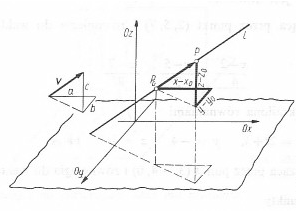
\includegraphics{rys/30_1.png}
	\caption{ }
	\label{fig:30.1}
\end{figure}
%TODO tutaj wstawić rysunek
Równanie to może być zapisane w postaciach:%\endinput
\begin{equation}
	x - x_0 = at, \quad y - y_0 = bt, \quad z - z_0 = ct, \qquad t \in \Re  \hfill \textrm{postać parametryczna}
	\label{eq30.2}
\end{equation}

\begin{equation}
	\frac{x - x_0}{a} = \frac{y - y_0}{b} = \frac{z - z_0}{c} \hfill \textrm{postać proporcji podwójnej}
	\label{eq30.3}
\end{equation}

\begin{equation}
	\begin{vmatrix}
		x - x_0 & y-y_0\\
		a & b
	\end{vmatrix}
	=
	\begin{vmatrix}
		y - y_0 & z - z_0\\
		b & c
	\end{vmatrix}
	=
	\begin{vmatrix}
		x - x_0 & z - z_0\\
		c & c
	\end{vmatrix}
	= 0 \hfill	\textrm{postać wyznacznikowa}
	\label{eq30.4}
\end{equation}

\begin{equation}
	\text{rząd} 
	\begin{bmatrix}
		x - x_0 & y - y_0 & z - z_0\\
		a & b & c
	\end{bmatrix}
	= 1	\hfill \textrm{zapis macierzowy}
	\label{eq30.5}
\end{equation}
\end{pkt}
\begin{dowod}
Każdy z powyższych warunków wyraża, że $P_0P||v$. Równoległość ta jest warunkiem koniecznym i wystarczającym na to, aby punkt $P$ leżał na prostej $l$.
\end{dowod}
\begin{uwaga}{1}
	Każdy z powyższych warunków jest równaniem prostej w przestrzeni $Oxyz$ wtedy i tylko wtedy, gdy $v \neq 0$, tzn. gdy co najmniej jedna z liczb $a$, $b$, $c$ jest różna od $0$.
\end{uwaga}
\begin{uwaga}{2}
	Zapis \ref{sec:30.3} odczytujemy w następujący sposób:\\
—	jeśli wszystkie trzy liczby $a$, $b$, $c$ są różne od $0$, zapis \ref{sec:30.3} jest równoważny układowi dwóch równań, dowolnie wybranych spośród trzech następujących równań

\begin{center}
$\frac{x - x_0}{a} = \frac{y - y_0}{b}, \qquad \frac{y - y_0}{b} = \frac{z - z_0}{c}, \qquad \frac{z - z_0}{c} = \frac{x - x_0}{a}$\\
\end{center}

—	jeśli jedna z liczb $a$, $b$, $c$ jest zerem, np. jeśli $b = 0$, to zapis \ref{sec:30.3} jest równoważny układowi dwóch równań
\begin{center}
$y - y_0 = 0, \qquad \frac{x - x_0}{a} = \frac{z - z_0}{c}$\\
\end{center}

—	jeśli dwie z liczb $a$, $b$, $c$ są zerami, np. jeśli $a = b = 0$, to zapis \ref{sec:30.3} jest równoważny układowi dwóch równań
\begin{center}
$x - x_0 = 0, \qquad y - y_0 = 0$\\
\end{center}

wówczas zmienna z jest dowolna.
\end{uwaga}

\begin{przyklad}{30.1}
Prosta przechodząca przez punkt $(2,5,7)$	i równoległa do wektora $[4,3,8]$ ma równanie
\begin{center}
$\frac{x - 2}{4} = \frac{y - 5}{3} = \frac{z - 7}{8}$\\
\end{center}
\end{przyklad}

\begin{przyklad}{30.2}
Jaka figura jest określona równaniami
\begin{center}
$x = 2t+3, \qquad y = -4, \qquad z = 5t \qquad t \in \Re$\\
\end{center}
Odp. Prosta przechodząca przez punkt $(3, —4, 0)$ i równoległa do wektora $[2, 0, 5]$.
\end{przyklad}
\\ \\
\textbf{Prosta przechodząca przez dwa punkty}\\
\begin{pkt}{30.2}
Prosta przechodząca przez dane dna różne punkty $P_0 = (x_0, y_0, z_0), P_1 = (x_1, y_1, z_1)$ ma równanie

\begin{equation}
	\stackrel{\rightarrow}{P_0P} = t\stackrel{\rightarrow}{P_0P_1} \qquad t \in \Re
	\label{eq:30.6}
\end{equation}

Równanie to może być zapisane w następujących postaciach:
\begin{equation}
	\begin{matrix}
	x - x_0 = t(x_1 - x_0)\\
	y - y_0 = t(y_1 - y_0)\\
	z - z_0 = t(z_1 - z_0)\\
	\end{matrix}
	\qquad	\textrm{t} \in \Re\\
	\label{eq:30.7}
\end{equation}
\end{pkt}

\begin{dowod}
Powyższe równania otrzymujemy z równań (\ref{eq:30.1})-(\ref{eq:30.3}), przyjmując $v = \stackrel{\rightarrow}{P_0P_1}$
\end{dowod}

\begin{przyklad}{30.3}
Napisać równanie przechodzącej przez punkty $(2,5,0)$ i $(3,5,7)$.\\
Otrzymujemy $\frac{x-2}{1} = \frac{y-5}{0}$, skąd $y=5, x-2=\frac{z}{7}$. Jest to prosta prostopadłado osi $O_y$
\end{przyklad}

\begin{odcinek}
Równanie odcinka otrzymujemy parametrycznych równań prostej przez stosowane ograniczenie zmienności parametru. Dołączając do równań (\ref{eq:30.7}) warunek $0\leq t \leq1$, otrzymujemy równanie odcinka $P_0P_1$. Równanie to możemy zapisać w postaci
\begin{equation}
	\begin{matrix}
	x = (1-t)x_0 + tx_1\\
	y = (1-t)y_0 + ty_1\\
	z = (1-t)z_0 + tz_1\\
	\end{matrix}
	\qquad	0 \leq t \leq 1
	\label{eq:30.9}
\end{equation}
\end{odcinek}
\\ \\
\textbf{Prosta i jej rzuty na płaszczyzny układu}\\
\begin{pkt}{30.3}
Równanie dowolnej prostej $l$, nie prostopadłej do $O_x$, mogą być napisane w postaci
\begin{equation}
	y = mx + p \quad z = nx + q
	\label{eq:30.10}
\end{equation}
Rzut $l'$ prostej l na płaszczyznę $O_x$$_y$ (rys. \ref{fig:30.2}) ma równania
\begin{equation}
	y = mx + p \quad z = 0
	\label{eq:30.11}
\end{equation}
%TODO tutaj rysunek 30.2
Rzut $l''$ prostej l na płaszczyznę $O_x$$_y$ ma równania
\begin{equation}
	y 0 \quad z nx + q
	\label{eq:30.12}
\end{equation}
W równaniach tych stałe $m$, $n$, $p$, $q$, mogą mieć wartości dowolne, zmienna $x$ przebiega przedział $(-\infty, \infty)$
\end{pkt}

\begin{dowod}
Pisząc równania parametryczne prostej $l$
\begin{equation}
	x = x_0 + at, \quad y=y_0 + bt, \quad z=z_0 + ct \qquad	\textrm{t} \in \Re
	\label{eq:30.13}
\end{equation}
mamy $a\neq0$. Wyliczając z pierwszego równania $t=(x-x_0)/a$ i wstawiając do pozostałych równań, otrzymujemy funkcje liniowe postaci (\ref{eq:30.10}). Przut $P'$ punktu $P=(x,y,z)$ na płaszczyznę $O_x$$_y$ na współrzędne $x$, $y$, $0$, skąd wynikaj równania (\ref{eq:30.11}). Rzut $P''$ punktu $P$ na płaszczyznę $O_x$$_z$ ma współrzędne $x$, $0$, $z$, skąd wynikają równania (\ref{eq:30.12}).
\end{dowod}

\section{Płaszczyzna w przestrzeni}{31}

\indent{Wyznaczanie płaszczyzny w przestrzeni jest możliwe na kilka sposobów. Podstawowym sposobem jest wskazanie jednego punktu płaszczyzny oraz kierunku, którego płaszczyzna jest prostopadła. Drugi sposób polega na wskazaniu jednego punktu płaszczyzny oraz dwóch różnych kierunków równoległych do tej płaszczyzny. Przejście od drugiego sposobu do pierwszego jest następujące: Jeżeli wektory $v_1, v_2$ są równoległe do płaszczyzny $G$ a nierównoległe jeden do drugiego, to wektor $N=v_1 x v_2$ jest wektorem niezerowym prostopadłym do płaszczyzny $G$.\newpage
Inne sposoby wyznaczania płaszczyzny - to wskazanie:

\begin{itemize}
	\item trzech punktów niekolinearnych lub
	\item dwóch prostych równoległych i różnych lub
	\item dwóch prostych przecinających się,\\
	przez które ma przechodzić ta płaszczyzna.
\end{itemize}
}
\textbf{Płaszczyzna przechodząca przez dany punkt i prostopadła do danego wektora}\\
\begin{pkt}{31.1}
Płaszczyzna $G$ przechodząca przez dany punkt $P_0=(x_0, y_0, z_0)$ i prostopadła do danego niezerowego wektora $N=[A, B, C]$ (rys. \ref{fig:31.1}) ma równanie
\begin{equation}
	N\cdot\stackrel{\rightarrow}{P_0P_1} = 0 \hfill	\textrm{postać wektorowa}\\
	\label{eq:31.1}
\end{equation}
W zapisie analitycznym równanie to ma postać
\begin{equation}
	A(x-x_0)+B(y-y_0)+C(z-z_0)=0 \hfill	\textrm{postać ogólna ukazująca jeden punkt płaszczyzny}
	\label{eq:31.2}
\end{equation}
\begin{figure}[ht]
	\centering
		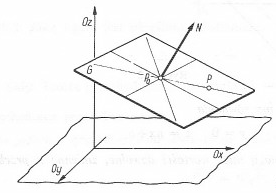
\includegraphics{rys/31_1.png}
	\caption{ }
	\label{fig:31.1}
\end{figure}
Oznaczając wielkość stałą $-Ax_0-By_0-Cz_0$ literą $D$, sprowadzamy równanie do postaci
\begin{equation}
	Ax+By+Cz+D=0 \hfill	\textrm{postać ogólna zredukowana}
	\label{eq:31.3}
\end{equation}
\end{pkt}
\begin{dowod}
Koniec P wektora $\stackrel{\rightarrow}{P_0P_1}$ leży w płaszczyźnie $G$ wtedy i tylko wtedy, gdy wektor ten jest prostopadły do wektora $N$, a więc zachodzi związek (\ref{eq:31.1}) oraz równoważne mu związki (\ref{eq:31.2}) i (\ref{eq:31.3})
\end{dowod}
\begin{uwaga}{1}
Każde z powyższych trzech równań jest równaniem płaszczyzny w przestrzeni $O_x$$_y$$z$ wtedy i tylko wtedy, gdy wektor $N$ jest niezerowy, tzn. gdy co najmniej jedna z liczb $A$, $B$, $C$ jest różna od $0$.
\end{uwaga}

\begin{przypadki}
Jeśli $A=0$, to $N \bot O_x$, zatem $G||O_x$. Jeśli $A=B=0$, to $N||O_z$, zatem $G \bot O_z$. Podobnie rozumujemy w pozostałych przypadkach tego rodzaju. Płaszczyzna $G$ przechodzi przez początek ikładu wtedy i tylko wtedy, gdy w równaniu ogólnym zredukowanym (\ref{eq:31.3}) wyraz wolny $D$ jest zerem.
\end{przypadki}

\begin{przyklad}{31.1}
Napisać równanie płaszczyzny $G$ symetralnej odcinka $M_1$ $M_2$ o końcach $M_1=(-2, 1, 7)$, $M_2=(4, 5, 3)$.
Płaszczyzna $G$ jest prostopadła do wektora $\bar{M_1M_2}=[6, 4, -4]$ i przechodzi przez środek $P_0$ odcinka $M_1$ $M_2$. Zgodnie z (\ref{eq:25.37}) mamy $P_0=(1,3,5)$. Płszczyzna $G$ ma więc równanie
\begin{equation}
	6(x - 1) + 4(y - 3) - 4(z - 5) = 0 \nonumber
\end{equation}
skąd po uproszczeniu i zredukowaniu dostajemy $3x+2y-2z+1=0$.
\end{przyklad}

\begin{przyklad}{31.2}
Wskazać wektor prostopadły do płaszczyzny
\begin{equation}
	G:4x + 5y + 6z = 60 \nonumber
\end{equation}
oraz jeden z punktów tej płaszczyzny.\\
Wektorem prostopadły do $G$ jest $N = [4, 5, 6]$. Dla $y = z = 0$ mamy $4z = 60$, więc $x = 15$. Punkt $(15, 0, 0)$ należy do G.
\end{przyklad}
\\ \\
\textbf{Płaszczyzna przechodząca przez dany punkt i równoległa do danych dwóch wektorów}
\begin{pkt}{31.2}
Płaszczyzna $G$ przechodząca przez dany punkt $P_0 = (x_0, y_0, z_0)$ i równoległa dwóch wektorów nierównoległych $v_1 = [a_1, b_1, c_1]$, $v_2 = [a_2, b_2, c_2]$ (rys. \ref{fig:31.2}) ma równanie
\begin{equation}
	\stackrel{\rightarrow}{P_0P_1} = tv_1+sv_2 \qquad	\textrm{t,s} \in \Re \hfill \textrm{postać parametryczna wektorowa}
	\label{eq:31.4}
\end{equation}
\begin{figure}[ht]
	\centering
		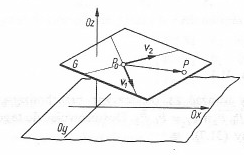
\includegraphics{rys/31_2.png}
	\caption{ }
	\label{fig:31.2}
\end{figure}
%str. 174 (pdf: str. 104)
Równanie to może być zapisane w następujących postaciach:
\begin{equation}
	\begin{matrix}
	x - x_0 = a_1t+a_2s\\
	y - y_0 = b_1t+b_2s\\
	z - z_0 = b_1t+b_2s\\
	\end{matrix}
	\qquad	\textrm{t} \in \Re \hfill \textrm{postać parametryczna}\\
	\label{eq:31.5}
\end{equation}
\begin{equation}
	\begin{vmatrix}
		x - x_0 & a_1 & a_2\\
		y - y_0 & b_1 & b_2\\
		z - z_0 & c_1 & c_2\\
	\end{vmatrix}
	= 0 \hfill	\textrm{postać wyznacznikowa}
	\label{eq:31.6}
\end{equation}
\end{pkt}
\begin{dowod}
Punkt $P$ leży na płaszczyźnie $G$ wtedy i tylko wtedy, gdy wektor $\stackrel{\rightarrow}{P_0P_1}$ jest komplanarny z wektorami $v_1V_2$, a więc gdy zachodzi związek (\ref{eq:31.4}) oraz równoważne mu związki (\ref{eq:31.5}) i (\ref{eq:31.6})
\end{dowod}

\begin{uwaga}{1}
Każde z równań (\ref{eq:31.4}) - (\ref{eq:31.6}) jest równaniem płaszczyzny wtedy i tylko wtedy, gdy wektory $v_1$, $v_2$ są nierównoległe.
\end{uwaga}

\begin{uwaga}{2}
Każdej parze wartości parametrów $t$, $s$ równania (\ref{eq:31.5}) przyporządkują (wzajemnie jednoznacznie) pewien punkt $P= (x,y,z)$ płaszczyzny $G$. Jeśli $s$ jest ustalone, a $t$ przebiega podział $(-\infty, \infty)$, to  $P$ przebiega pewną prostą zawartą w $G$ i równoległą do wektora $v_1$. Na odwrót, przy $t$ ustalonym, a $s$ zmiennym punkt $P$ kreśli na $G$ prostą równoległą do $v_2$.
\end{uwaga}

\begin{uwaga}{3}
Równanie (\ref{eq:31.6}) możemy sprowadzić do postaci (\ref{eq:31.2}) rozwijając wyznacznik według pierwszej kolumny
\end{uwaga}

\begin{przyklad}{31.3}
Co przedstawiają równania parametryczne
\begin{equation}
	x=2t-3s, \quad y=t+s+2, \quad z=1-s, \qquad \textrm{t} \in \Re
	\label{eq:31.5}
\end{equation}
Odp. Płaszczyznę równoległą do wektorów $[2, 1, 0]$, $[-3, 1, -1]$ i przechodzą przez punkt $(0, 2, 1)$
\end{przyklad}
\\ \\
\textbf{Płaszczyzna przechodząca przez 3 dane punkty}
\begin{pkt}{31.3}
Płaszczyzna $G$ przechodząca przez 3 dane niekolinearne punkty $P_0=(x_0, y_0, z_0), P_1= (x_1, y_1, z_1), P_2=(x_2, y_2, z_2)$ ma równanie
\begin{equation}
	\begin{vmatrix}
		x - x_0 & x_1-x_0 & x_2-x_0\\
		y - y_0 & y_1-y_0 & y_2-x_0\\
		z - z_0 & z_1-z_0 & z_2-x_0\\
	\end{vmatrix}
	= 0 \hfill	\textrm{płaszczyzna przez 3 punkty}
	\label{eq:31.7}
\end{equation}
\begin{figure}[ht]
	\centering
		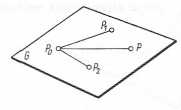
\includegraphics{rys/31_3.png}
	\caption{ }
	\label{fig:31.3}
\end{figure}
\end{pkt}

\begin{dowod}
Płaszczyznę, $G$ (rys. \ref{fig:31.7}) możemy uważać za płaszczyznę przechodzącą przez $P_0$ i równoległą do wektorów $v_1 = \stackrel{\rightarrow}{P_0P_1}$ i $v_2 = \stackrel{\rightarrow}{P_0P_2}$. Dostosowując do tego przypadku, równanie (\ref{eq:31.6}) otrzymujemy (\ref{eq:31.7}).
\end{dowod}

\begin{uwaga}{1}
Równanie (\ref{eq:31.7}) może być zapisane w postaci
\begin{equation}
	\begin{vmatrix}
		x & x_0 & x_1 & x_2\\
		y & y_0 & y_1 & y_2\\
		z & z_0 & z_1 & z_2\\
		1 & 1 & 1 & 1
	\end{vmatrix}
	= 0 \hfill	\textrm{płaszczyzna przez 3 punkty}
	\label{eq:31.7}
\end{equation}
Dla sprawdzenia tego wystarczy odjąć drugą kolumnę od pozostałych, po czym rozwiązać wyznacznik według czwartego wiersza.\\
Za pomocą transpozycji powyższych wyznaczników możemy uzyskać to, że zmienne $x, y, z$ znajdą się w pierwszym wierszu.
\end{uwaga}
\\ \\
\textbf{Płaszczyzna przechodząca przez 2 proste równoległe}
\begin{pkt}{31.4}
Płąszczyzna $G$ zawierająca dwie proste $l_0, l_1$ równoległe i różne, dane równaniami
\begin{equation}
	l_0: \frac{x - x_0}{a} = \frac{y - y_0}{b} = \frac{z - z_0}{c} \quad l_1: \frac{x - x_1}{a} = \frac{y - y_1}{b} = \frac{z - z_1}{c}
\end{equation}
ma równanie 
\begin{equation}
	\begin{vmatrix}
		x - x_0 & a & x_1 - x_0\\
		y - y_0 & b & y_1 - y_0\\
		z - z_0 & c & z_1 - z_0\\
	\end{vmatrix}
	= 0 
	\label{eq:31.8}
\end{equation}
\begin{figure}[ht]
	\centering
		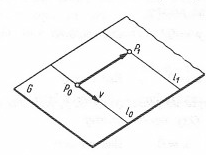
\includegraphics{rys/31_4.png}
	\caption{ }
	\label{fig:31.4}
\end{figure}
\end{pkt}

\begin{dowod}
(rys. \ref{fig:31.4}). Jest płaszczyzna przechodząca przez punkt $P_0= (x_0, y_0, z_0), P_0 \in l_0$ i równoległa do wektorów $v=[a, b, c]$ i $\stackrel{\rightarrow}{P_0P_1}$, gdzie $P_1 \in l_1$, np. $P_1 = (x_1, y_1, z_1)$. Stosując do tego przypadku równanie (\ref{eq:31.6}), dostajemy (\ref{eq:31.7}). 
\\ \\
\textbf{Płaszczyzna zawierająca prostą $l_1$ i równoległą do prostej $l_2$}
\end{dowod}

\begin{pkt}{31.5}
Jeżeli proste $l_1$, $l_2$, wzajemnie nierównoległe, są dane równaniami
\begin{equation}
	l_0: \frac{x - x_0}{a} = \frac{y - y_0}{b} = \frac{z - z_0}{c} \quad l_1: \frac{x - x_1}{a} = \frac{y - y_1}{b} = \frac{z - z_1}{c}
\end{equation}
to płaszczyzna $G$ zawierająca prostą $l_1$ i równoległa do prostej $l_2$, ma równanie
\begin{equation}
	\begin{vmatrix}
		x - x_1 & a_1 & x_2 - x_0\\
		y - y_1 & b_1 & y_2 - y_0\\
		z - z_1 & c_1 & z_2 - z_0\\
	\end{vmatrix}
	= 0 
	\label{eq:31.9}
\end{equation}
\end{pkt}

\begin{dowod}
Jest to płaszczyzna przechodząca przez punkt $P_1 = (x_1, y_1, z_1)$ i równoległa do wektorów $v_1 = [a_1, b_1, c_1]$ i $v_2 = [a_2, b_2, c_2]$. Pisząc dla tego przypadku równanie (\ref{eq:31.6}), dostajemy (\ref{eq:31.9}).
\end{dowod}
\\ \\
%str. 176 (pdf: str. 106)
\textbf{Postać kierunkowa równania płaszczyzny}

\begin{pkt}{31.6}
	Dowolna płaszczyzna nierównoległa do osi $Oz$ może być przedstawiana równaniem
\begin{equation}
	z=ax+by+c \hfill	\textrm{płaszczyzna przez 3 punkty}
	\label{eq:31.10}
\end{equation}
i na odwrót, dla dowolnie obranych wartości $a, b, c$ równanie to przedstawia pewną płaszczyznę nierównoległą do osi $Oz$ (rys. \ref{fig:31.5})
\begin{figure}[ht]
	\centering
		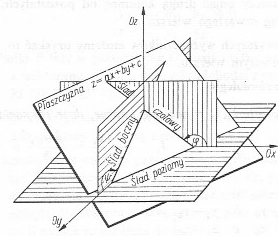
\includegraphics{rys/31_5.png}
	\caption{ }
	\label{fig:31.5}
\end{figure}
Płaszczyzna (\ref{eq:31.10}) przecina płaszczyznę $Oxz$ wzdłuż prostej
\begin{equation}
	z=ax+c \quad y=0 \hfill	\textrm{ślad czołowy}
	\label{eq:31.11}
\end{equation}
oraz płaszczyznę $Oyz$ wzdłuż prostej
\begin{equation}
	z=by+c \quad x=0 \hfill	\textrm{ślad boczny}
	\label{eq:31.12}
\end{equation}
Jeśli $a = b = 0$, to płaszczyzna (\ref{eq:31.10}) jest równoległa do płaszczyzny $Ozy$, jeśli zaś $a\neq 0$ lub $b\neq 0$, to płaszczyzna (\ref{eq:31.10}) przecina płaszczyznę $Ozy$ wzdłuż prostej
\begin{equation}
	ax + by + c = 0 \quad z=0 \hfill	\textrm{ślad poziomy}
	\label{eq:31.13}
\end{equation}
\end{pkt}
\begin{dowod}
Dowolna płaszczyzna ma równanie $A_x + B_y + C_z + D = 0$. Jeśli jest to płaszczyzna nierównoległa do osi $O_z4$, to $C \neq 0$, zatem $z = - \frac{A}{C}x - \frac{B}{C}y - \frac{D}{C}$. Oznaczając $a = - \frac{A}{C}$, $b = - \frac{B}{C}$, $c = - \frac{D}{C}$, otrzymujemy równanie (\ref{eq:31.10}).\\
Na odwrót, równanie (\ref{eq:31.10}) można sprowadzić do postaci $ax + by - z + c = 0$, skąd widać, że jest to równanie płaszczyzny prostopadłej do wektora $[a, b, -1]$ a więc nierównoległej do osi $O_z$. \\
Punkt wspólny płaszczyzny (\ref{eq:31.10}) i płaszczyzny $Oxz$ spełnia koniunkcję równać $z = ax + by + c$, $y = 0$. Koniunkcja ta jest równoważna warunkowi (\ref{eq:31.11}). Podobnie uzasadniamy resztę tezy.
\end{dowod}
\begin{uwaga}{}
Współczynniki $a, b$ w równaniu (\ref{eq:31.10}) są współczynnikami kierunkowymi śladów tej płaszczyzny na ścianach układu $Oxyz$ (rys. \ref{fig:31.5})
\begin{equation}
	a = tg\varphi \quad b = tg\psi
	\label{eq:31.14}
\end{equation}
dlatego o równaniu (\ref{eq:31.10}) mówimy, że ma postać kierunkową.
\end{uwaga}

\begin{pkt}{31.7}
Jeśli płaszczyzna o równaniu
\begin{equation}
	z=ax+by+c
	\label{eq:31.15}
\end{equation}
przechodzi przez punkt $(x_0, y_0, z_0)$, to równanie jej może być napisane w postaci
\begin{equation}
	z - z_0 = a(x - x_0) + b(y-y_0)
	\label{eq:31.16}
\end{equation}
\end{pkt}
\begin{dowod}
Mamy równość prawdziwą $z_0 = ax_0 + by_0 + c$. Odejmując ją od (\ref{eq:31.15}), dostajemy (\ref{eq:31.16}).
\end{dowod}
\\ \\
\textbf{Postać odcinkowa równania płaszczyzny}
\begin{pkt}{31.7}
Płaszczyzna odcinająca na osiach układu $Oxyz$ niezerowe wektory $\stackrel{\rightarrow}{OA},\stackrel{\rightarrow}{OB},\stackrel{\rightarrow}{OC}$ o miarach $a$, $b$, $c$ ma równanie
\begin{equation}
	\frac{x}{a} + \frac{y}{b} + \frac{z}{c} = 0 \hfill	\textrm{postać odcinkowa}
	\label{eq:31.17}
\end{equation}
Dowód analogiczny do dowodu twierdzenia \ref{tw:28.5}
\end{pkt}
\begin{uwaga}{}
Równanie płaszczyzny może być napisane w postaci odcinkowej, jeśli płaszczyzna przecina wszystkie 3 osie układu i nie przechodzi przez początek układu.
\end{uwaga}
\\ \\
\textbf{Postać normalna równania płaszczyzny}
\begin{pkt}{31.8}
Niech będzie dana półprosta $n$, której początkiem jest początek układu i która tworzy z osiami składu $Oxyz$ kąty kierunkowe o miarach $\alpha = {x,n}$, $\beta = {y,n}$, $\gamma = {z,n}$. Płaszczyzna $G$ prostopadła do półprostej $n$ i odcinająca na niej odcinek długości $h$, $h \geq 0$, ma równanie
\begin{equation}
	x cos\alpha + y cos\beta + z cos \gamma - h = 0 \hfill	\textrm{postać normalna (Hessego)}
	\label{eq:31.18}
\end{equation}
Dowód i uwaga - analogicznie jak przy twierdzeniu 28.6 
\end{pkt}

\section{Zagadnienia dotyczące prostej i płaszczyzny w przestrzeni}{32}

\textbf{Kąt dwóch prostych w przestrzeni.} Kątem prostych $l_1, l_2$
\begin{center}
$< \{l_1, l_2\}$
\end{center}
nazywamy kąt dwóch niezerowych wektorów $u_1$, $u_2$ (\ref{fig:32.1}) obranych w ten sposób, żeby $u_1||l_1$, $u_2||l_2$ i żeby kąt wektorów $u_1$, $u_2$ miał miarę łukową nie większą od $\pi/2$ (spełnienie tego ostatniego warunku uzyskujemy przez ewentualną zmianę zwrotu wektora). Miarę kąta prostych $l_1$, $l_2$ oznaczamy $\{l_1, l_2\}$.

\begin{figure}[ht]
	\centering
		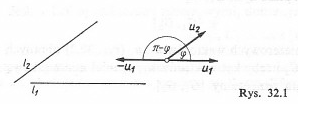
\includegraphics{rys/32_1.png}
	\caption{ }
	\label{fig:31.3}
\end{figure}

W przypadku prostych przecinających się powyższa definicja jest zgodna z definicją na str. 164. Kąt prostych równoległych, względnie pokrywających się, ma miarę $0$. \\
Jeśli $v_1$, $v_2$ są dowolnymi wektorami niezerowymi, równoległymi odpowiednio do prostych $l_1$,$l_2$ to
\begin{equation}
	cos \{l_1,l_2\} = |cos\{v_1, v_2\}|, sin \{l_1,l_2\} = |sin\{v_1, v_2\}| \nonumber
\end{equation}

\begin{przyklad}{32.1}
Wyznaczyć cosinus kąta prostych $l_1$, $l_2$ danych równaniami
\begin{equation}
	l_1: \frac{x}{2} = \frac{y}{3} = \frac{z - 1}{4} \qquad l_2: \frac{x - 6}{3} = \frac{y +8}{-4} = \frac{z}{5} \nonumber
\end{equation}
Z równań odczytujemy $v_1$ = [2,3,4], $v_2$ = [3,-4,5], zatem 
\begin{equation}
cos \{l_1,l_2\} = \frac{|2\cdot3+3\cdot(-4)+4\cdot5|}{\sqrt{2^2+3^2+4^2} \sqrt{3^2+(-4)^2+5^2}} = \frac{14}{\sqrt{29}\sqrt{50}} \nonumber
\end{equation}
\end{przyklad}

\begin{przyklad}{32.2}
Jaki kąt tworzą proste $l_1$,$l_2$ dane równaniami
\begin{equation}
	l_1: \frac{x}{2} = \frac{y}{3} = \frac{z - 1}{9} \qquad l_2: \frac{x - 6}{3} = \frac{y +8}{4} = \frac{z}{-2} \nonumber
\end{equation}
Mamy $v_1 = [2,3,9]$, $v_2$ = [3,4,-2], cos \{$v_1$,$v_2$\} = 0, \{$l_1$,$l_2$\} = $\pi/2$, $l_1 \bot l_2$
\end{przyklad}

\begin{przyklad}{32.3}
Wyznacz kąt prostych $l_1$,$l_2$ danych równaniami
\begin{equation}
	l_1: \frac{x-1}{-2} = \frac{y}{3} = \frac{z}{-5} \qquad l_2: y = -\frac{3}{2}x, z = \frac{5}{2}x+1 \nonumber
\end{equation}
Mamy $v_1 = [-2,3,-5]$. Równanie prostej $l_2$ sprowadzamy do prostej parametrycznej. Przyjmując $x-2t$, mamy $y=-3t$,$z=5t+1$. Zatem $v_2=[-2,3,-5]$. Ponieważ $v_1||v_2$, więc $l_1||l_2$.
\end{przyklad}

\textbf{Punkt wspólny dwóch prostych.} Aby stwierdzić czy proste $l_1$,$l_2$ mają punkt wspólny, należy zbadać czy istnieje trójka liczb $x$, $y$, $z$ spełniają równania obu prostych. W tym celu z równań jednej prostej wyrażamy dwie zmienne przez trzecią i podstawiamy do równań drugiej prostej. Jeśli otrzymany układ jest rozwiązany, to punkt wspólny istnieje, jeśli otrzymany układ jest sprzeczny, to punkt wspólny nie istnieje.

\begin{przyklad}{32.4}
Zbadać czy istnieje punkt wspólny prostych $l_1$, $l_2$ w przykładzie 32.2 \\
Z równań $l_1$ wyliczamy $y=\frac{3}{2}x$, $z=\frac{9}{2}x+1$. Wstawiając tak wyznaczone $y$ i $z$ do równań $l_2$, otrzymamy układ sprzeczny. Proste $l_1$, $l_2$ nie mają punktu wspólnego
\end{przyklad}
\textbf{Kąt dwóch płaszczyzn.}Kątem dwóch płaszczyzn $G_1$, $G_2$
\begin{center}
$<$ \{$G_1$, $G_2$\}
\end{center}
nazywamy kąt dwóch niezerowych wektorów $u_1$, $u_2$ (\ref{fig:32.2}) obranych w ten sposób, żeby $u_1 \bot G$, $u_2 \bot G$ i żeby kąt wektoru $u_1$, $u_2$ miał miarę łukową nie większą od $\pi/2$. Miarę tego kąta oznaczamy \{$G_1$, $G_2$\}.

\begin{figure}[ht]
	\centering
		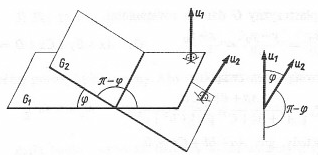
\includegraphics{rys/32_2.png}
	\caption{Kąt między płaszczyznami i kąt między wektorami prostopadłymi do tych płaszczyzn}
	\label{fig:31.3}
\end{figure}

Jeśli $N_1$, $N_2$ są dowolnymi wektorami niezerowymi, prostopadłymi odpowiednio do płaszczyzn $G_1$, $G_2$, to
\begin{equation}
	cos \{G_1, G_2\} = |cos \{N_1, N_2\}|, \quad sin \{G_1, G_2\} = sin \{N_1, N_2\}  \nonumber
\end{equation}

\begin{przyklad}{32.5}
Wyznacz kąt dwóch płaszczyzn w przypadkach:\\
a) $x+y-z=0$, \quad $2x+3y+4z+5=0$\\
b) $x+y-z=0$, \quad $4x-3y+z+9=0$\\
c) $x+2y-3z+8=0$, \quad $2x+4y-6z+19=0$\\
Rozwiązanie. a) $N_1=[1,1,-1]$, $N_2=[2,3,4]$, $cos\{N_1, N_2\}=1/\sqrt{87}$ miara stopniowa kąta płaszczyzn wynosi $83^o51'$\\
b) płaszczyzny prostopadłe;\quad c) płaszczyzny równoległe.
\end{przyklad}
\textbf{Kąt prostej i płaszczyzny.} Niech $l$ będzie prostą, $G$ - płaszczyzną, a $n$ - prostą prostopadłą do $G$. Kąt prostej $l$ i płaszczyzny $G$
\begin{center}
$< \{l, G$\}
\end{center}
definiujemy jako dopełnienie kąta prostych $l$, $n$ do kąta prostego

\begin{figure}[ht]
	\centering
		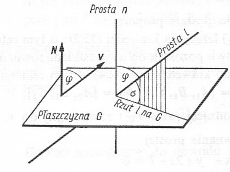
\includegraphics{rys/32_3.png}
	\caption{ }
	\label{fig:31.3}
\end{figure}

Mamy więc związki
\begin{equation}
	\{l, G\} = \frac{\pi}{2} - \{l, n\}|, \quad sin \{l, G\} = cos \{l, n\}  \nonumber
\end{equation}
Jeśli $v$ i $N$ są wektorami niezerowymi, dodatnimi tak, że $v||l, N \bot G$ (\ref{fig:32.3}), to
\begin{equation}
sin \{l,G\} = |cos\{v,N\}|
\end{equation}

\begin{przyklad}{32.6} Kąt prostej $l$ i płaszczyzny $G$ danych równaniami
\begin{equation}
	l: \frac{x-x_0}{a} = \frac{y-y_0}{b} = \frac{z-z+0}{c} \qquad G: A_x+B_y+C_z+D=0 \nonumber
\end{equation}
ma miarę $\delta$ wyznaczoną przez związki
\begin{equation}
	sin\delta= \frac{|Aa+Bb+Cc}{\sqrt{A^2+B^2+C^2}\sqrt{a^2+b^2+c^2}}, \qquad 0\leq\delta\leq\frac{\pi}{2}
	\label{eq:32.1}
\end{equation}
$l||G$ wtedy i tylko wtedy, gdy $Aa+Bb+Cc=0$
\end{przyklad}
\textbf{Prosta jako krawędź przecięcia się dwóch płaszczyzn}
\begin{pkt}{32.1}
Jeśli każde z równań
\begin{equation}
	\begin{matrix}
	A_1x+B_1y+C_1z+D_1=0\\
	A_2x+B_2y+C_2z+D_2=0\\
	\end{matrix}
	\qquad \textrm{postać krawędziowa równania prostej}
	\label{eq:32.2}
\end{equation}
przedstawia prostą stanowiącą krawędź przecięcia się tych dwóch płaszczyzn.

\begin{figure}[ht]
	\centering
		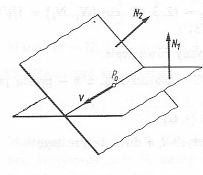
\includegraphics{rys/32_4.png}
	\caption{ }
	\label{fig:31.3}
\end{figure}

Przejście od postaci krawędziowej do postaci proporcji:\\
1) znajdujemy punkt $P_0=(x_0,y_0,z_0)$ leżący na krawędzi (\ref{eq:32.2}); w tym celu można jedną współrzędną obrać dowolnie, a dwie pozostałe obliczyć z układu równań (\ref{eq:32.2});\\
2) znajdujemy wektor $v$ równoległy do krawędzi (\ref{fig:32.4}) w tym celu najprościej jest przyjąć $v= N_1xN_2$, gdzie $N_1=[A_1,B_1,C_1]$, $N_2=[A_2,B_2,C_3]$;\\
3) piszemy równanie prostej przechodzącej przez $P_0$ i równoległej do $v$.
\end{pkt}
\begin{przyklad}
Napisać w postaci proporcji równanie prostej
\begin{equation}
l:
\begin{matrix}
3x-y+2z-7=0\\
x+3y-2z+3=0
\end{matrix}
\nonumber
\end{equation}
Rozwiązanie. 1) Obierając $x=0$, otrzymujemy z równań prostej $y=2$, $z= \frac{9}{2}$,\\ więc $P_0=(0,2,\frac{9}{2})$.\\
2)Przyjmujemy
\begin{equation}
v=N_1xN_2=
\begin{vmatrix}
i & j & k \\
3 & -1 & 2 \\
1 & 3 & -2 \\
\end{vmatrix}
= [-4,8,10]
\end{equation}
3) Prosta $l$ ma równanie
\begin{equation}
\frac{x}{-4}=\frac{y-2}{8}=\frac{z-9/2}{10}
\end{equation}
\end{przyklad}
\end{document}